\documentclass[paper=a4, fontsize=11pt]{scrartcl}
\usepackage[left=25mm,top=30mm,right=25mm,bottom=30mm]{geometry}
\usepackage{titling}
\usepackage{dirtytalk}
\usepackage{mathtools}
\usepackage{multirow}
\DeclarePairedDelimiter{\ceil}{\lceil}{\rceil}
    
    \date{}
    \setlength{\droptitle}{-10em}
    \title{\textbf{Raport tema nr 2}}

\begin{document}

\maketitle
\vspace{-6em}
\section{Descrierea problemei}
\paragraph{}
Să se implementeze un algoritm genetic care să minimizeze următoarele funcții: 
\break \textit{Rastrigin}, \textit{Griewangk}, \textit{Rosenbrock}, \textit{De Jong}.

\section{Algoritmul utilizat}
\paragraph{}
Pentru rezolvarea acestei probleme, vom implementa un algoritm genetic, care are la bază
o strategie evolutivă, plecând de la o populație inițială de cromozomi care, pe măsură ce avansează,
evoluează cu ajutorul operatorilor genetici.

\subparagraph{2.1}
Detalii de implementare

\paragraph{}
\underline{\smash{Reprezentarea soluțiilor}} a fost făcută pe șiruri binare, astfel: 
\say{Spaţiul de căutare se va disctretiza până la o anumită precizie $10^{-d}$. 
Un interval [a, b] va fi împărţit în N = $(b-a)*(10^d)$ subintervale egale.
Pentru a putea reprezenta cele $(b-a)*(10^d)$ valori, este nevoie de un număr n = $\ceil{log_2N}$ de biţi.
Lungimea şirului de biţi care reprezintă o soluţie candidat va fi suma lungimilor reprezentărilor pentru fiecare parametru al funcţiei de optimizat. În momentul evaluării soluției (apelul funcției de optimizat) este necesară decodificarea fiecărui parametru reprezentat ca șir de biți în număr real, după formula: $X_{real} = a + decimal(x_{biti})*(b-a)/(2^n-1)$.}

Populația este reprezentată în memorie printr-o matrice care reține mai mulți cromozomi, fiecare cromozom fiind un șir de biți.

\underline{\smash{Inițializarea}} constă în crearea random a unor cromozomi reprezentați binar. 

\underline{\smash{Funcția fitness}} este utilizată pentru a măsura calitatea cromozomilor. Ea este formulată plecând de la funcția numerică de optimizat. Trebuie să fie pozitivă și este construită pentru maximizare.

Scopul \underline{\smash{selecției}} este de a alege pentru supraviețuire cei mai adaptați indivizi din populație cu speranța că descendenții acestora vor avea un fitness mai ridicat.
O presiune de selecție ridicată duce la crearea unei diversități scăzute în populația creată.
Pe de altă parte, o presiune de selecție scazută încetinește evoluția.
În algoritmul implementat este folosită schema de selecție "Roata norocului".

\underline{\smash{Operatorii genetici}} folosiți sunt mutația (modificarea unei gene alese aleatoriu) și încrucișarea (schimbul de informație genetică între doi cromozomi).

\subparagraph{2.1}
Pseudocod

\begin{enumerate}
    \itemsep0em
    \item[1.] Se generează random o populație inițială.
    \item[2.] Cât timp populația evoluează:
    \begin{enumerate}
        \item[a)] Se evaluează populația curentă.
        \item[b)] Se selectează cromozomii pentru următoarea generație.
        \item[c)] Cromozomii se supun încrucișării și mutației.
    \end{enumerate} 
    \item[3.] Se returnează cea mai bună soluție găsită.
\end{enumerate}

\vspace{40mm}
\section{Rezultate experimentale}

\begin{table}[h]
    \begin{tabular}{|l|l|l|l|l|l|l|}
    \hline
    Algoritm                                                                      & Funcție                                                       & Nr dimensiuni & Nr rulări            & Minim      & Medie      & Maxim      \\ \hline
    \multirow{10}{*}{\begin{tabular}[c]{@{}l@{}}Algoritm \\ Genetic\end{tabular}} & \multirow{3}{*}{Rastrigin}                                    & 5             & \multirow{10}{*}{15} & 3.103      & 4.663      & 5.666      \\ 
                                                                                  &                                                               & 10            &                      & 25.55      & 37.38      & 46.78      \\
                                                                                  &                                                               & 30            &                      & 146.3      & 185.6      & 220.8      \\ \cline{2-3} \cline{5-7}
                                                                                  & \multirow{3}{*}{Griewank}                                     & 5             &                      & 0.0004     & 0.0029     & 0.0063     \\
                                                                                  &                                                               & 10            &                      & 0.129      & 0.183      & 0.214      \\
                                                                                  &                                                               & 30            &                      & 0.643      & 0.807      & 0.89       \\ \cline{2-3} \cline{5-7}
                                                                                  & \multirow{3}{*}{Rosenbrock}                                   & 5             &                      & 4.073      & 7.765      & 12.19      \\
                                                                                  &                                                               & 10            &                      & 53.37      & 112.4      & 142.4      \\
                                                                                  &                                                               & 30            &                      & 3674       & 8365       & 12737      \\ \cline{2-3} \cline{5-7}
                                                                                  & \multirow{3}{*}{De Jong}                                      & 5             &                      & 0.021      & 0.068      & 0.135      \\ 
                                                                                  &                                                               & 10            &                      & 2.712      & 3.381      & 4.126      \\
                                                                                  &                                                               & 30            &                      & 16.49      & 27.74      & 37.87      \\ \hline
    \end{tabular}
\end{table}


\begin{table}[h!]
    \resizebox{1.1\textwidth}{!}{\begin{tabular}{|l|l|l|l|l|l|l|l|l|}
    \hline
    \multicolumn{2}{|c|}{Algoritm}                                                                 & \multicolumn{1}{r|}{Functie testată}                                           & Nr dimensiuni & Nr rulări                  & Minim    & Medie    & Maxim    & Deviație \\ \hline
    \multicolumn{2}{|l|}{\multirow{12}{*}{\begin{tabular}[c]{@{}l@{}}Simulated\\ Annealing\end{tabular}}} & \multirow{3}{*}{De Jong}                                                       & 5             & \multirow{3}{*}{30}        & 1.49     & 4.01     & 7.117    & 4.2         \\ 
    \multicolumn{2}{|l|}{}                                                                                &                                                                                & 10            &                            & 7.89     & 23.7     & 32.6     & 10         \\ 
    \multicolumn{2}{|l|}{}                                                                                &                                                                                & 30            &                            & 98.07    & 145.9    & 162.1    & 15.68         \\ \cline{3-9} 
    \multicolumn{2}{|l|}{}                                                                                & \multirow{3}{*}{Rastrigin}                                                     & 5             & \multirow{3}{*}{30}        & 13.7     & 25.7     & 38.08    & 16.96         \\ 
    \multicolumn{2}{|l|}{}                                                                                &                                                                                & 10            &                            & 65.17    & 93.85    & 106.6    & 15.82         \\
    \multicolumn{2}{|l|}{}                                                                                &                                                                                & 30            &                            & 360.9    & 392.6    & 423.7    & 16.25         \\ \cline{3-9} 
    \multicolumn{2}{|l|}{}                                                                                & \multirow{3}{*}{Schwefel 7}                                                    & 5             & \multirow{3}{*}{30}        & -1642    & -1247    & 0        & 354.4         \\  
    \multicolumn{2}{|l|}{}                                                                                &                                                                                & 10            &                            & -2361    & -1820    & 0        & 440         \\  
    \multicolumn{2}{|l|}{}                                                                                &                                                                                & 30            &                            & -5417    & -3266    & 0        & 594.9         \\ \cline{3-9} 
    \multicolumn{2}{|l|}{}                                                                                & \multirow{3}{*}{\begin{tabular}[c]{@{}l@{}}Six-hump\\ camel back\end{tabular}}                                                        & \multirow{3}{*}{2}             & \multirow{3}{*}{30}        & \multirow{3}{*}{-1.03}      & \multirow{3}{*}{-1}      & \multirow{3}{*}{0}      & \multirow{3}{*}{0.16}         \\  
    \multicolumn{2}{|l|}{}                                                                                &                                                                                &               &                            &       &       &       &          \\  
    \multicolumn{2}{|l|}{}                                                                                &                                                                                &               &                            &       &       &       &          \\ \hline
    \end{tabular}}
\end{table}


\begin{table}[h!]
    \resizebox{1.12\textwidth}{!}{\begin{tabular}{|l|l|l|l|l|l|l|l|l|l|l|l|l|}
    \hline
    \multicolumn{2}{|c|}{Algoritm}                 & \multicolumn{1}{|c|}{Funcție}                                              & Dimensiuni & Rulări                  & Minim    & Medie   & Maxim  & Deviație          & Minim   & Medie    & Maxim   & Deviație       \\ \hline
    \multicolumn{5}{|l|}{}                                                                                                                                             & \multicolumn{4}{|c|}{Best Improvement}          & \multicolumn{4}{|c|}{First Improvement}       \\ \hline
    \multicolumn{2}{|l|}{\multirow{12}{*}{\begin{tabular}[c]{@{}l@{}}Hill\\ Climbing\end{tabular}}} & \multirow{3}{*}{De Jong}  & 5          & \multirow{3}{*}{30}     & 1.204    & 4.647   & 9.574  & 4.966             & 1.137    & 4.296   & 8.205   & 5.987          \\
    \multicolumn{2}{|l|}{}                          &                                                                           & 10         &                         & 10.44    & 23.24   & 34.67  & 12.28             & 14.69    & 25.40   & 41.40   & 9.950          \\ 
    \multicolumn{2}{|l|}{}                          &                                                                           & 30         &                         & 98.07    & 145.3   & 168.8  & 20.53             & 134.2    & 149.7   & 169.2   & 8.969          \\ \cline{3-13} 
    \multicolumn{2}{|l|}{}                          & \multirow{3}{*}{Rastrigin}                                                & 5          & \multirow{3}{*}{30}     & 14.21    & 30.57   & 43.29  & 18.54             & 14.21    & 30.20   & 39.74   & 14.49          \\  
    \multicolumn{2}{|l|}{}                          &                                                                           & 10         &                         & 68.71    & 93.05   & 114.2  & 18.50             & 66.86    & 96.10   & 116.2   & 21.05          \\  
    \multicolumn{2}{|l|}{}                          &                                                                           & 30         &                         & 337.5    & 390.8   & 423.1  & 24.60             & 335.9    & 392.3   & 417.1   & 18.74          \\ \cline{3-13} 
    \multicolumn{2}{|l|}{}                          & \multirow{3}{*}{Schwefel 7}                                               & 5          & \multirow{3}{*}{30}     & -1801    & -1260   & 0      & 505               & -1810    & -1188   & 0       & 457.5          \\  
    \multicolumn{2}{|l|}{}                          &                                                                           & 10         &                         & -2128    & -1871   & 0      & 186.8             & -2714    & -1909   & 0       & 329.6          \\ 
    \multicolumn{2}{|l|}{}                          &                                                                           & 30         &                         & -5525    & -5489   & 0      & 51.47             & -5529    & -5499   & 0       & 38.92          \\ \cline{3-13} 
    \multicolumn{2}{|l|}{}                          & \multirow{3}{*}{\begin{tabular}[c]{@{}l@{}}Six-hump\\ camel back\end{tabular}} & \multirow{3}{*}{2}              & \multirow{3}{*}{30}     & \multirow{3}{*}{-1.02}        & \multirow{3}{*}{-0.95}        & \multirow{3}{*}{0}       & \multirow{3}{*}{0.38}          & \multirow{3}{*}{-1.03}         & \multirow{3}{*}{-0.96}       & \multirow{3}{*}{0}       & \multirow{3}{*}{0.235}          \\ 
    \multicolumn{2}{|l|}{}                          &                                                                           &            &           &             &          &         &        &        &          &        &           \\  
    \multicolumn{2}{|l|}{}                          &                                                                           &            &           &             &          &         &        &        &          &        &           \\ \hline
    \end{tabular}}
\end{table}

\vspace{10mm}
\paragraph{}
Rezultatele algoritmului genetic au fost obținute cu o populație inițială de 100 de cromozomi, pe 100 de iterații, 1000 generații,
$P\_CROSS = 0.3$ și $P\_MUTATION = 0.1$.

În ultimele două tabele se pot observa valorile obținute cu algoritmii \textit{Hill Climbing} și \textit{Simulated Annealing}.

Observăm o îmbunătățire la funcțiile \textit{Rastrigin} și \textit{De Jong}, ajungându-se foarte aproape de minimul lor global.

\underline{\smash{Influența valorilor parametrilor}}: Dacă mutația sau încrucișarea cromozomilor se realizează prea des, un individ nu poate evolua la fel de bine,
pentru că ar ajunge să fie complet diferit. Astfel, dacă mărim $P\_MUTATION$ la $0.5$, vom obține rezultate mai slabe (de exemplu, minimul pentru Rastrigin cu 5 dimensiuni
va fi $3.8$).
De asemenea, cu cât lăsăm populația să evolueze mai mult, cu atât o să obținem rezultate mai bune.

\begin{figure}[h!]
    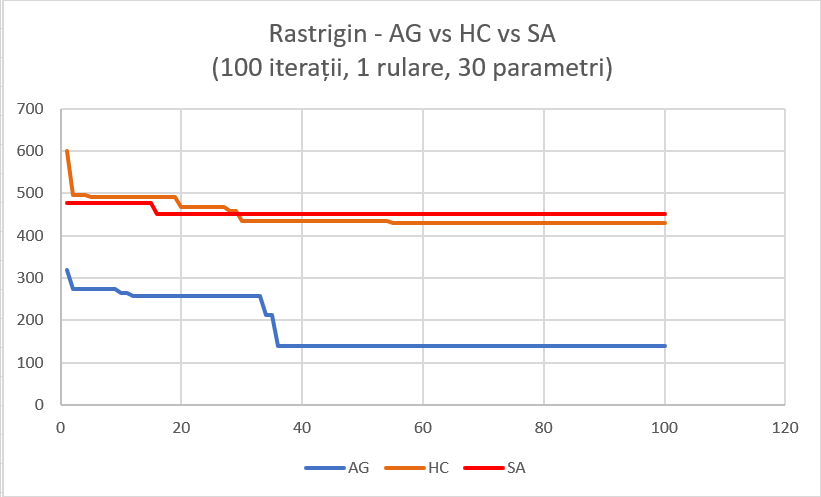
\includegraphics[scale=0.9]{GraficRastrigin.png}
\end{figure}

\begin{figure}[h]
    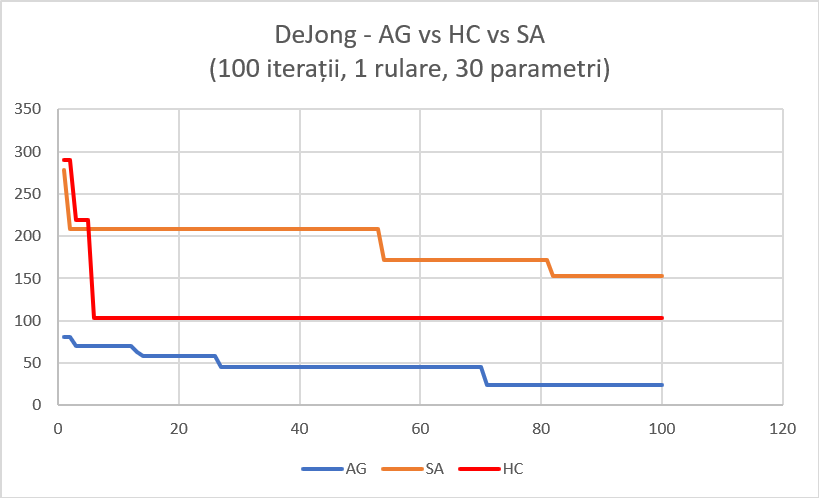
\includegraphics[scale=0.9]{GraficDeJong.png}
\end{figure}

\end{document}